$K$-Nearest Neighbours ($K$NN), as the name suggests, is the process of finding $K$ nearest neighbours to a given query point. In this project, the $K$NN query is only performed on 2-dimensional data. In addition, we only use $\ell_2$ norm as the distance metric. A $K$NN query will be formalised as $\mathcal{K}(\boldsymbol{X})$ where $\boldsymbol{X}\in\mathbb{R}^2$.

\subsubsection{$K$NN query with $K$D-Tree}

As a baseline, we first perform $K$NN query with $K$D-tree.

\begin{figure}[htp]
    \centering
    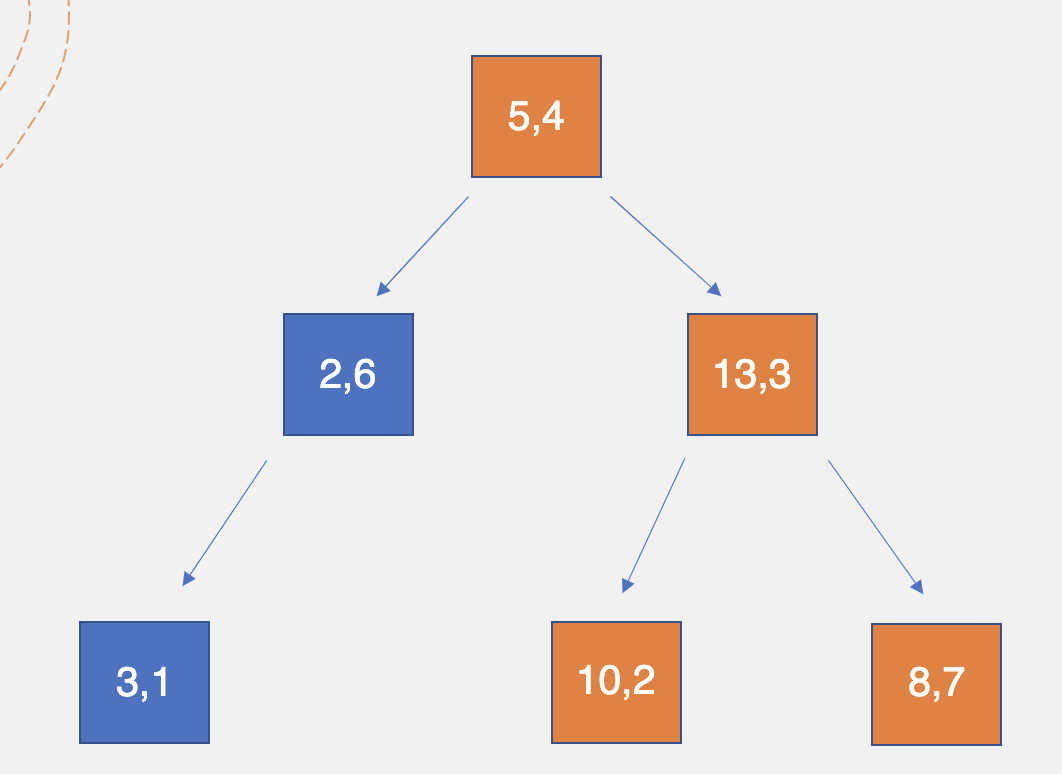
\includegraphics[width=0.4\textwidth]{graphs/KD-Tree_KNN_Tree.png}
    \caption{$K$D-Tree for KNN Query}
    \label{fig:$K$D-Tree_for_KNN Query}
\end{figure}

\begin{figure}[htp]
    \centering
    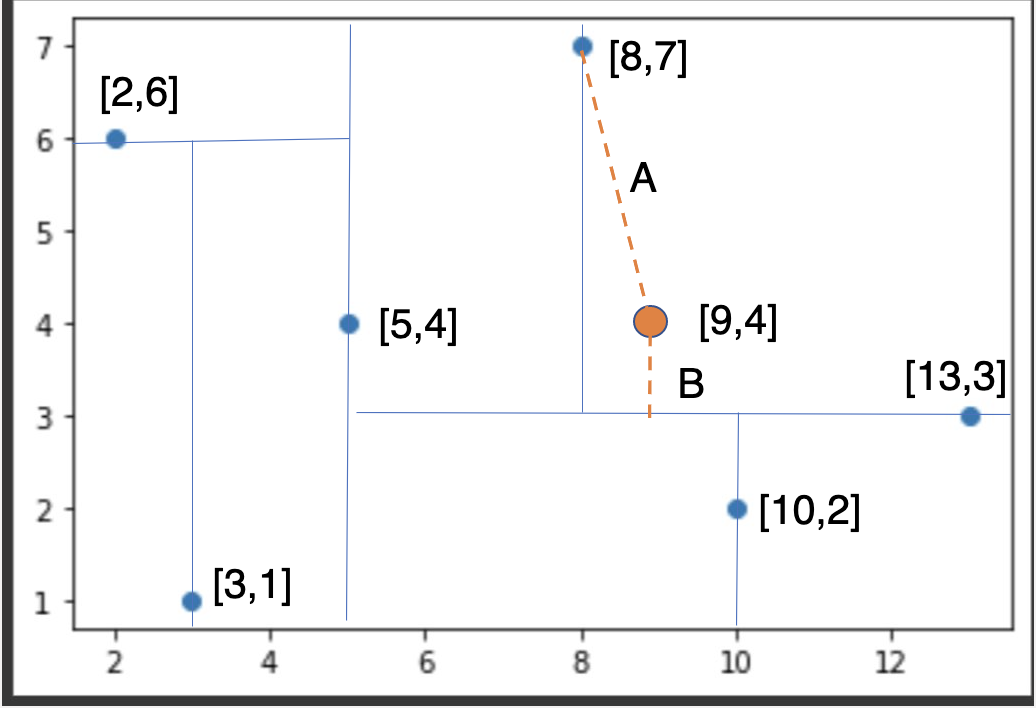
\includegraphics[width=0.6\textwidth]{graphs/KD-Tree_KNN_plot.png}
    \caption{$K$D-Tree KNN Plot on 2-dimentional plane}
    \label{fig:KD_Tree_KNN_Plot}
\end{figure}


\begin{mscexample}
	For example, we have Point list as $((5,4),(2,6),(13,3),(8,7),(3,1),(10,2))]$ then we will have a tree structure as shown in \ref{fig:$K$D-Tree_for_KNN Query} and it's plot on $2$-dimensional plane is shown in \ref{fig:KD_Tree_KNN_Plot}. As we can see in \ref{fig:KD_Tree_KNN_Plot} that even though point $(8,7)$ is the leaf we will reach when we traverse the tree to search for point nearest to test point $(9,4)$ it is not infact the nearest point to the test data. In this case if we want to look for $4$ nearest neighbour, we first check the square of euclidean distance of $(9,4)$ with the root of the tree i.e., $(5,4)$ which is $16$. It then calculates the distance with $(2,6)$ and $(13,3)$ which calculates to $53$ and $17$ respectively. It then keeps traversing to the right node while calculating distance until it reaches a leaf. After reaching the leaf it then checks the distance with $(8,7)$ with a distance of $10$ which is infact smaller than the previous shortest distance of 16 with the root. It adds these points to the list. It then makes a decision weather to go left from $(13,3)$ based on the distance of the test point with leaf $(8,7)$ i.e., A and the perpendicular distance with point $(13,3)$ which is B. Since distance A > B as can be seen in the figure \ref{fig:KD_Tree_KNN_Plot} there is a chance that there could a point in the subtree with a distance smaller than the previous points. In this case it will then check the distance with point $(10,2)$ and the distance is the shortest(best distance) so far of $5$. 
\end{mscexample}



\subsubsection{$K$NN Query with LISA}
We do not know the analytical representation of shards, as we use machine learning model $ \mathcal{SP}$ to generate shards. Thus,it is difficult to apply traditional KNN query pruning strategies applicable for KD-Trees, to LISA model. 

Consider a query point $q_{knn}=x=(x_{0},x_{1})$, let $x^{'} \in V$ be the Kth nearest key to x in database at a distance value $\delta = \| x^{'}-x\|_{2} $. Lets define $ \mathcal{Q}(x,\delta) \triangleq [x_{0}-\delta, x_{0}+\delta) \times[x_{1}-\delta, x_{1}+\delta)$ and $\mathcal{B}(x, \delta)  \triangleq \{p \in V \mid \| x-p\|_{2} \leq \delta \} $.We can create a query rectangle $qr =  \mathcal{Q}(x, \delta + \epsilon)$ where $\epsilon \rightarrow 0$. As shown in Fig. \ref{fig:KNN_Query_Lisa}, K nearest keys to x are all in $\mathcal{B}(x, \delta)$ and thus in qr. KNN query can be solved using the range query if we can estimate an appropriate distance bound $\delta$ for every query point.

\begin{figure*}[t]
    \centering
    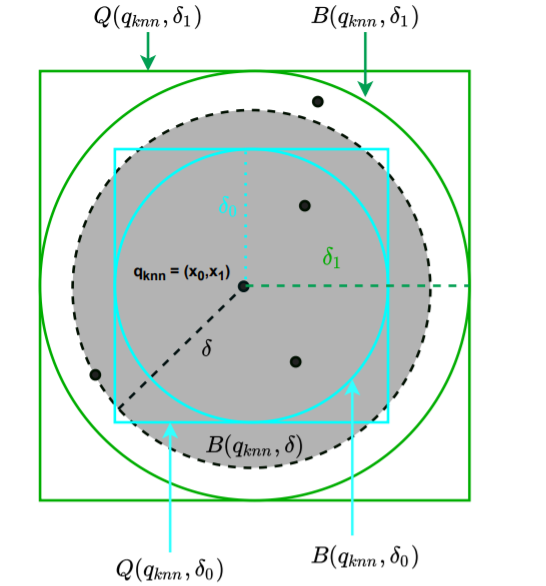
\includegraphics[width=0.7\textwidth]{graphs/KNN_Query_Lisa.png}
    \caption{KNN Query Implementation in Lisa(K=3)\\
    1)$q_{knn}$ represents the query point, $ \mathcal{Q}(x,\delta) \triangleq [x_{0}-\delta, x_{0}+\delta) \times[x_{1}-\delta, x_{1}+\delta)$, represents query rectangle and $ \mathcal{B}(x, \delta)$ represents the key space at distance $\delta$ containing K nearest keys.\\
    2)KNN query can be solved by range query if we can estimate an appropriate distance bound $\delta$ for every query point\\
    }
    \label{fig:KNN_Query_Lisa}
\end{figure*}